\documentclass[11pt]{article}
\usepackage[utf8]{inputenc}
\usepackage[T1]{fontenc}
\usepackage{babel}
\usepackage{amsmath}
\usepackage{graphicx}
\usepackage{fancyhdr}
\usepackage{algorithmic} 
\usepackage{algorithm}
\pagestyle{fancy}
\usepackage{tcolorbox}
\usepackage{rotating} 
\usepackage{multirow}
\usepackage{caption}
\usepackage{blindtext}
\usepackage{tabularx,ragged2e}
\newcolumntype{C}{>{\Centering\arraybackslash}X} % centered "X" column
\usepackage[toc,page]{appendix}
\fancyhf{}
\renewcommand{\headrulewidth}{0pt}
\setlength{\headheight}{40pt} 
\pagestyle{plain}
\usepackage{lineno}
\linespread{1.2}
%% Sets page size and margins
\usepackage[letterpaper,top=3cm,bottom=3cm,left=3cm,right=3cm,marginparwidth=1.75cm]{geometry}

\title{Implementing and Optimizing Stochastic Gradient Descent Hmailton Monte Carlo Method}
\author{Rihui Ou(ro49),Tianhui Zhou
(tz47) }

\documentclass{article}


\begin{document}



\maketitle

\section{Abstract}
\paragraph{}
Compared with regular MCMC method, Hamilton Monte Carlo (HMC), can explore the posterior space more efficiently by modeling the posterior sampling as some physics system. However, as the number of data and dimension grow, the gradient calculation and Metropolis-Hasting correction contained in the algorithm can be quite painful as a curse of dimensionality. Yet, another published paper\cite{chen2014stochastic}, proposed a methods called Stochastic Gradient Hamiltonian Monte Carlo (SGHMC), which talked about how to circumvent the full gradient calculation and metropolis hasting correction by only doing stochastic gradient and introducing some noises. In this project, we realized their method, tried to optimize it, and applied it to data. We also compared the outcome of this methods with two other methods:one is the HMC method without Metropolis–Hastings (M-H), the other is Stochastic Langevin Dynamics (SGLD). Of three algorithms we used, the HMC method without M-H correction was the most naive and we used it as baseline. The SGHMC was the main algorithm we studied. It turned out that SGHMC was quite efficient in exploring the posterior space in both our simulated data set and real data set in terms of the prediction performance using posterior predicted distribution.

\section{Background}
\paragraph{}
Hamilton Monte Carlo (HMC), a gradient-based MCMC method, is an alternative method to classical MCMC methods with attractive properties such as faster exploration of the state space. However, HMC scales poorly when we are faced with massive data set as computing the gradient of a Hamilton system becomes intractable in this case. To ease the scalable problem, this project adpoted a method which introduced a noisy gradient estimate based on the so-called minibatch method instead of the full gradient in every iteration\cite{chen2014stochastic}. Although this method is inevitably injected with noises, it brings substantial computational gains especially when making inference on data sets with redundant information.

The paper we used introduced a friction term into the Hamilton system, which they showed can counteract the effect of noise. Moreover, it circumvents the costly Metropolis-Hasting step in the traditional HMC method. However, this method has its disadvantages,too. Introducing a new term means that there are extra parameters to tune, which is often based on some "rules of thumb". 


\section{Description of Algorithm}
\paragraph{}
Our goal is to sample $\theta$ from 
\begin{align}
    p(\theta | \mathcal{D}) \propto \exp (-U(\theta)) \label{eq:post}
\end{align}
where $\theta$ is the parameter of interest and $\mathcal{D}$ is the data,  and the potential function $U$ is defined by
$$U=-\sum_{x \in \mathcal{D}} \log p(x | \theta)-\log p(\theta)
$$
To sample from \eqref{eq:post}, HMC defines a Hamilton system through introducing an auxiliary variable momentum $r$. In other words, HMC samples from the joint system:
\begin{equation}
    \pi(\theta, r) \propto \exp \left(-U(\theta)-\frac{1}{2} r^{T} M^{-1} r\right)
\end{equation}
instead and then discards the samples of $r$. HMC simulates the following Hamilton dynamics:
\begin{equation}
    \left\{\begin{array}{l}{d \theta=M^{-1} r d t} \\ {d r=-\nabla U(\theta) d t}\end{array}\right. \label{ham}
\end{equation}
where $M$ is the mass matrix, often set to be an identity matrix. Typically we discretize the system in \eqref{ham} to obtain the HMC algorithm, which is displayed in Algorithm 1(\textbf{benchmark algorithm}). 
\begin{algorithm}
	\caption{Hamilton Monte Carlo without M-H steps}
	\label{ALG:HMC}
	\begin{algorithmic} 
		\REQUIRE The initial point $\theta_0$ and stepsize $\epsilon$
		\FOR{$t=0,1,\cdots$}
        \STATE Resample momentum variable $r$ from $N(0,M)$ and set it to be $r^{(t)}$
        \STATE $\left(\theta_{0}, r_{0}\right)=\left(\theta^{(t)}, r^{(t)}\right)$
        \STATE Update $r_{0} \leftarrow r_{0}-\frac{\epsilon}{2} \nabla \tilde{U}(\theta)$
        \FOR{$i=1,\cdots,m$}
            \STATE $\theta_{i} \leftarrow \theta_{i-1}+\epsilon M^{-1} r_{i-1}$
            \STATE $r_{i}\leftarrow r_{i-1}-\epsilon \nabla \tilde{U}(\theta)$
        \ENDFOR
        \STATE Set $\theta^{(t+1)}\leftarrow\theta_m$ 
		\ENDFOR
	\end{algorithmic}
\end{algorithm}

However, as mentioned before, due to the scalability of the data, computing the full gradient $\nabla U(\theta)$ is often intractable. To implement Algorithm \ref{ALG:HMC}, a common practice is to use a noisy gradient estimate $\nabla \tilde{U}(\theta)$ instead of $\nabla U(\theta)$:
\begin{equation}
    \nabla \tilde{U}(\theta)=-\frac{|\mathcal{D}|}{|\tilde{\mathcal{D}}|} \sum_{x \in \mathcal{D}} \nabla \log p(x | \theta)-\nabla \log p(\theta), \tilde{\mathcal{D}} \subset \mathcal{D}\label{eq:noi}
\end{equation}
In equation \eqref{eq:noi},  $\tilde{\mathcal{D}}$, the minibatch, is a subset sampled uniformly from the data $\mathcal{D}$. In other words, the full gradient $\nabla U(\theta)$ is estimated based on the subset $\tilde{\mathcal{D}}$. However, this method is inaccurate in theory, since we neither used the full gradient nor the M-H correction. But we will use it to serve as a benchmark to see how wrong can this method be if the problem got complicated. This method would be referred to as MHC without M-H in following sections.


A method proposed by \cite{welling2011bayesian} is based on the first order Langevin dynamics(SGLD). This method does not include the momentum variable $r$ and takes gradient directly. The details of this algorithm is shown in Algorithm \ref{ALG:SGLD}(\textbf{comparison algorithm}).
\begin{algorithm}
	\caption{Stochastic Gradient Langevin Dynamics}
	\label{ALG:SGLD}
	\begin{algorithmic} 
		\REQUIRE The initial point $\theta_0$ and stepsize $\epsilon$
		\FOR{$t=0,1,\cdots$}
        \STATE update $\theta^{(k+1)} \leftarrow \theta^{(k)}-\epsilon \cdot \nabla \tilde{U}(\theta)+\mathcal{N}\left(0,2 \epsilon I\right)$
		\ENDFOR
	\end{algorithmic}
\end{algorithm}

In practice, a friction term can be introduced into the Hamilton system to reflect the second-order Langevin dynamics, as shown in \eqref{eq:fri}. 
\begin{equation}
    \left\{\begin{aligned} d \theta=& M^{-1} r d t \\ d r=&-\nabla U(\theta) d t-C M^{-1} r d t \\ &+\mathcal{N}(0,2(C-\hat{B}) d t)+\mathcal{N}(0,2 B d t) \end{aligned}\right. \label{eq:fri}
\end{equation}

Using the similar method to discretize the system \eqref{eq:fri}, we have the stochastic gradient descent Hamilton Monte Carlo (SGHMC) algorithm \cite{chen2014stochastic}, which is the principal algorithm used in this report. This algorithm is shown in Algorithm \ref{ALG:SGHMC}(\textbf{main algorithm}).
\begin{algorithm}
	\caption{Stochastic Gradient Hamilton Monte Carlo}
	\label{ALG:SGHMC}
	\begin{algorithmic} 
		\REQUIRE The initial point $\theta_0$ and stepsize $\epsilon$
		\FOR{$t=0,1,\cdots$}
        \STATE $\left(\theta_{0}, r_{0}\right)=\left(\theta^{(t)}, r^{(t)}\right)$
        \STATE Update $r_{0} \leftarrow r_{0}-\frac{\epsilon}{2} \nabla U\left(\theta_{0}\right)$
        \FOR{$i=1,\cdots,m$}
            \STATE $\theta_{i} \leftarrow \theta_{i-1}+\epsilon M^{-1} r_{i-1}$
            \STATE $r_{i} \leftarrow r_{i-1}-\epsilon \nabla \tilde{U}\left(\theta_{i}\right)-\epsilon C M^{-1} r_{i-1}+\mathcal{N}\left(0,2(C-\hat{B}) \epsilon\right)$
        \ENDFOR
        \STATE Set $\left(\theta^{(t+1)}, r^{(t+1)}\right)=\left(\theta_{m}, r_{m}\right)$ 
		\ENDFOR
	\end{algorithmic}
\end{algorithm}

\newpage
\section{Describe optimization for performance}
\paragraph{}
As was written in the stochastic gradient HMC algorithm, to resample momentum $r$ every m steps is not mandatory. The whole system is added with friction, so it is not moving on a contour with same total energy if we do not resample momentum. Then the whole function just involves a single loop. Unlike other sampling method for posterior, this method does not require M-H evaluation at the end of each loop, which gives another boost to the speed. That means the algorithm, even written in plain python, is already a very fast one. 

Since the whole algorithm involves passing a user defined gradient function as one of its argument, therefore, the optimization could have some restriction. If we want to use Pybind \cite{moldovan2016pybinding} or Cython\cite{behnel2011cython} optimization, it is quite difficult to incorporate a plain python function into a C++ based structure. Therefore, we only applied Numba\cite{lam2015numba} as our optimization strategy. In our case, the nopython option is unavailable due to the same reason, since passing a unknown user defined function not recognized by Numba can fail the type inference. Hence, the only place that Numba helped was to accelerate the speed of loops.
We also modified some small places in original code like using np.linalg.solve  instead np.linalg.inv to solve matrix inversion to gain more stability, avoiding doing repetitive matrix inversion when some result can be saved and reused. After the modification, we tested on two small simulation cases. 

\textbf{Case 1}:This is the case from the original paper where we assumed that the $U(\theta)=2\times\theta^2-\theta^4$  

Using the regular python to generate 300000 sample:      

 1.52 s $\pm$ 18.4 ms per loop (mean $\pm$ std. dev. of 7 runs, 1 loop each)


Using the Numba optimized function to generate 300000 sample:  

1.45 s $\pm$ 14.2 ms per loop (mean $\pm$ std. dev. of 7 runs, 1 loop each)

\textbf{Case 2:}
It is a multivariate normal case, where we assumed that the posterior density follows normal distribution with mean 0 and variance: 
$
\begin{bmatrix} 
1 & 0.9& 0.8\\
0.9 & 1 &0.9\\
0.8 &0.9&1\\
\end{bmatrix}
$

Using the plain python to generate 30000 sample:  

9.08 s $\pm$ 32.1 ms per loop (mean $\pm$ std. dev. of 7 runs, 1 loop each)

Using the numba optimized function to generate 30000 sample:  

 7.52 s $\pm$ 49.9 ms per loop (mean $\pm$ std. dev. of 7 runs, 1 loop each)


Since the higher dimension involves more matrix operation, and currently, we can not use nopython mode to further optimize the data structure, hence the Numba only boosted loops here as well.

In both case, we only witnessed tiny improvement, that was probably because the limitation of data structure, and the extra time needed for Numba compilation. However, the raw regular python code is already impressive enough to draw 30000 posterior three dimensional samples within 10 seconds, given that all programs were run on a relatively incapable server. The fast sampling should largely be attributed to this efficient sampling algorithm for posterior distribution.

\section{Comparative analysis with competing algorithms}
\paragraph{}
In this paper, we mainly compared the SGHMC  with two other algorithms, one is the HMC without M-H, the other is SGLD as was discussed in the description of algorithm section. Since all three algorithms involves similar logic, we coded them all by ourselves. 
The comparison mainly focused on prediction on test data based on posterior predictive distribution. We compared the relationship between number of iterations and test error on both simulated data sets and real data sets, and the results were presented in the following two sections.

Moreover, we conducted a simple numerical experiment to examine the ability to explore spaces of both the SGLD and SGHMC algorithm. We use both algorithms to sample from a bivariate Gaussian distribution. Here, the mean of this Gaussian distribution is $(0,0)^T$ and the covariance is 
$
\begin{bmatrix} 
1 & 0.95\\
0.95 & 1 \\
\end{bmatrix}
$. Moreover, the gradient is injected with a $N(0,I_2)$ noise.


According to \cite{chen2014stochastic}, the momentum variable $r$ can drive the sampler to move along the contour. Therefore, the SGHMC sampler is more efficient to explore the parameter space especially when the parameters follow a highly correlated distribution. As shown in Figure \ref{fig:corr}, the samples of SGHMC samplers are more concentrated on the high density region, indicating a better performance.

\begin{figure}[h!]
\centering
\caption{First 100 samples of SGHMC and SGLD}
\label{fig:corr}
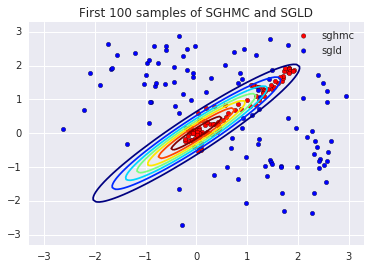
\includegraphics[scale=0.5]{mini.png}
\end{figure}

\section{Applications to simulated data sets }
\paragraph{}
First, we tested the performance of all three algorithms on a simulated logistics regression dataset. We generate a 20000 by 5 data matrix, with each entry following an i.i.d $N(0,1)$ distribution. Then, we set the true value of $\theta$ to be $(2,10,-5,0,0)^T$, and simulate $y_i$ from $Bin(1,p_i)$, where $p_i$ is $\frac{1}{1+exp(-x_i^T\theta)}$ and $x_i$ is the $i$ th row of $X$.

In this simulated data example, since the simulated process was based on the underlying relation between the log odds of outcome and covariates to follows a linear relationship. Our sampler took a minibatch of size 200 per iteration, the overall result was quite good.
This result showed similar pattern compared with the experiment of original paper done on MNIST data\cite{chen2014stochastic}, which was a extension of logistic regression.
As was shown in Figure \ref{fig:Figure1}, all three methods reached about 90$\%$ accuracy after 500 iterations. In the long term, SGLD has the best accuracy. SGDHMC and SGLD are similar both in convergence speed and final accuracy, about 93$\%$. HMC without M-H is much slower and its final accuracy is about 92$\%$.

\begin{figure}[h!]
\centering
\caption{Test Error for Three Algorithms on Simulated Data}
\label{fig:Figure1}
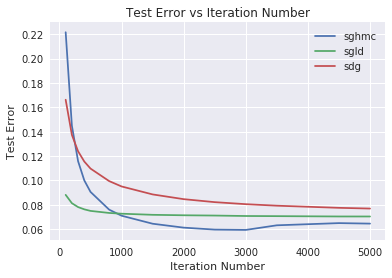
\includegraphics[scale=0.5]{simu.png}
\end{figure}

\section{Applications to real data sets}
\paragraph{}
We used the US Adult Income dataset, taken from \url{https://www.kaggle.com/johnolafenwa/us-census-data}, to test the performance of our previously mentioned algorithm. This dataset was extracted from the 1994 US Census dataset consisting of covariates such as race, native country and so on. The response variable is whether the income of each subject exceeds 50K USD. We built a logistics regression model to study how various factors impact subjects' income.

We adapted some code from Kaggle to preprocess the dataset. All preprocessing details are available in \url{https://www.kaggle.com/kost13/us-income-logistic-regression}. However, there are some difference between the preprocessing procedure in Kaggle and my practice. I dropped all categorical variables, deleted missing values and did not transform some variables into categorical ones. Eventually, 7 covariates were left and below is the description:
\begin{itemize}
    \item Age: the age of each individual
    \item fnlgwt: final weight
    \item Education Num: the number of years subjects attend schools
    \item Sex: 0 stands for male, 1 stands for female
    \item Capital Gain: income from investment
    \item Capital Loss: loss from investment
    \item Hours/Week: the working hours of each subject per week
\end{itemize}

The application to real data sets followed exactly what were done for simulated data. Only in this case, we had no idea what the underlying data generation process was. We could fit a Bayesian deep neural network as was done in the example from paper, or SVM\cite{welling2011bayesian}, which was also very efficient in classification. However, we still fit a regular logistic model, due to the limited computation resources and the fact that logistic model is one of the the most naive and simplest resolution to binary classification problem. . 

In this case, none of those models did quite satisfactory prediction for the outcome as was shown in \ref{fig:Figure2}. It could happen due to many reasons, such as predictors are not informative enough(we left out some missing information and categorical variables); the relationship was nonlinear and so on. However, it did gave us some clue of how those three model worked under a real data situation.
Similar to what we have seen in simulated data set SGLD and SGHMC had quick convergence and can finally reach an accuracy for about 73$\%$. In this case, however, the HMC without M-H method deviated a lot from truth. In theory, the HMC without M-H method was not correct, as was mentioned before. We just wanted to use it as a benchmark to see how things might go wrong when the situation got more complicated. Here, the result was like a fail coin toss game, which means that this method did a terrible job exploring the posterior space in this case.


\begin{figure}[h!]
\centering
\caption{Test Error for Three Algorithms on Real Data}
\label{fig:Figure2}
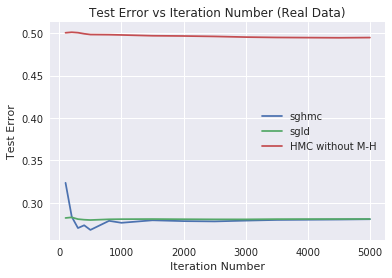
\includegraphics[scale=0.5]{real.png}
\end{figure}




\section{Discussion and Conclusion}
\paragraph{}
By comparing SGHMC with two other methods, we had some practical evidence that this method can efficiently explore the posterior space, especially when $\theta$ follows a highly correlated distribution. For simulated data, it can reach an overall accuracy of about 93$\%$ then stayed stable after drawing about 2000 posterior samples. For real data, it can reach an overall accuracy of about 73$\%$ then stayed stable after drawing about 1000 posterior samples. 


The method compared with other method, has its unique merit in exploring the posterior space. It not only inherits the property of efficient exploring the space by regular HMC, but also, it only needs to calculate the gradient on minibatch of data, and it does not require to do MH evaluation at the end of each draw. All those merits have given the method a extraordinary gain in speed. The code from git for the original paper was written in plain matlab, and since the algorithm is already fast enough, the author did not deliberately try to optimize it.
In our process of optimization, there is one small obstacle, the gradient needs to be passed as an argument to the function.
Due to the difficulty of passing a user defined function written in python in to a cython or pybind type function. We simply applied numba to facilitate the calculation. We can see that both in 1d posterior or higher dimensional parameter space, we achieved visible but not substantial marginal gain in speed.   

Due to the previous constraints in passing functions, and also considering that defining a gradient function is not always easy for user when dimension of parameter goes higher,the future plan to improve the function might include:
\begin{itemize}
    \item Build the whole algorithm under neural network in tensor flow, which automatically does numerical gradient
    \item Incorporate a series of default modes into the function: linear regression, logistic regression so that user does not need to define the gradient function when dealing with regular settings.
\end{itemize}
\bibliographystyle{apalike}
\bibliography{ref}
\end{document}
